\providecommand{\main}{../../..}
\documentclass[\main/main.tex]{subfiles}
\begin{document}

\subsection{Esercizio 7}
Si determini la soluzione ottima con la funzione di utilità $u = \w_1f_1 + \w_2f_2$ con $\w_1 = 0.25$ e $\w_2 = 0.75$ del seguente problema di programmazione a due obbiettivi:

\begin{figure}
  \begin{align*}
    \max f_1 = -x_1 + 2x_2 \\
    \max f_1 = 2x_1 - x_2  \\
    x_1 + x_2  & \leq 7    \\
    -x_1 + x_2 & \leq 3    \\
    x_1 - x_2  & \leq 3    \\
    x_1, x_2   & \leq 4    \\
    x_1, x_2   & \geq 0
  \end{align*}
  \caption{Esercizio 7}
\end{figure}

Si supponga ora di aggiungere un terzo obbiettivo, anch'esso da massimizzare $f_3 = 2x_1 + x_2$ e si disegnino nel piano $\w_1-\w_2$ le regioni nelle quali ciascuna soluzione di base ammissibile del problema lineare risulta ottima.

\subsection{Soluzione esercizio 7}

\subsubsection*{Costruisco funzione obbiettivo}

\[
  u = 0.25(-x_1 + 2x_2) + 0.75(2x_1-x_2) = 1.25x_1 + 0.75x_2
\]
\subsubsection*{Risolvo il problema lineare con la nuova funzione obbiettivo}

\begin{align*}
  u^* = 1.25x_1 - 0.25x_2 \\
  x_1 + x_2  & \leq 7     \\
  -x_1 + x_2 & \leq 3     \\
  x_1 - x_2  & \leq 3     \\
  x_1, x_2   & \leq 4     \\
  x_1, x_2   & \geq 0
\end{align*}
La variabile con cofficiente massimo è $x_1$, che può assumere al massimo valore $4$. Il valore di $x_2$ è invece da minimizzare, e può assumere valore minimo $1$ se fissiamo $x_1=4$.

\subsubsection*{Verifico la soluzione}

\begin{figure}
  \begin{subfigure}{0.45\textwidth}
    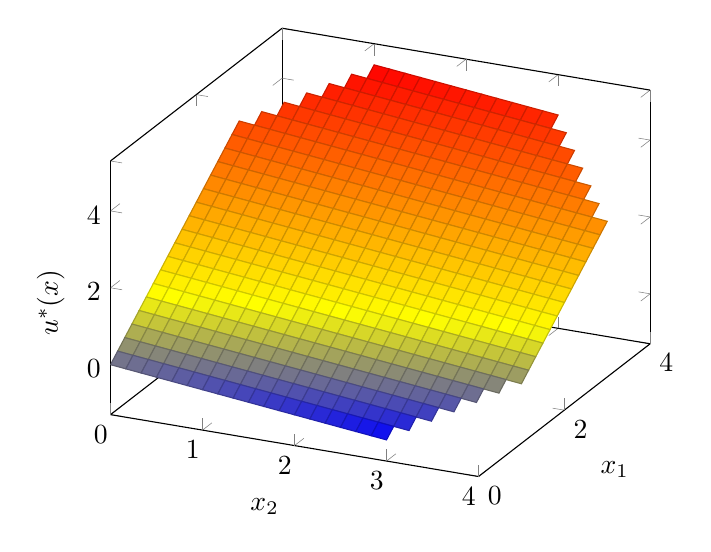
\begin{tikzpicture}
      \begin{axis}[
          xlabel=$x_2$,
          ylabel=$x_1$,
          zlabel=$u^*(x)$,
          domain=0:4,
          y domain=0:4
        ]
        \addplot3[surf, unbounded coords=jump]
        {x+y<=7 && x-y <= 3 && -x+y <= 3 ? 1.25*y - 0.25*x : NaN};
      \end{axis}
    \end{tikzpicture}
    \caption{La funzione $u^*(x)$}
  \end{subfigure}
  ~
  \begin{subfigure}{0.45\textwidth}
    \includegraphics[width=0.8\textwidth]{es7-maut}
    \caption{Dominio della funzione $u^*(x)$}
  \end{subfigure}
\end{figure}

\subsubsection*{Aggiungo funzione obbiettivo aggiuntiva}
Considerando il peso di $w_3 = 1- \w_1 - \w_2$ e $\w_1+\w_2\leq1$, procedo ad identificare le soluzioni ottime al variare dei pesi.

La nuova funzione obbiettivo risulta:

\[
  u' = \w_1(-x_1 + 2x_2) + \w_2(2x_1 - x_2) + (1 - \w_1 -\w_2)(2x_1 + x_2) = \w_1(-3x_1 + x_2) - 2\w_2x_2 + 2x_1 + x_2
\]

\begin{figure}
  \includegraphics[width=0.4\textwidth]{es7-maut}
  \caption{Area di definizione}
\end{figure}

I vertici sono in $v_1 = (0,3), v_2 = (1,4), v_3 = (3,4), v_4=(4,3), v_5=(4,1), v_6=(3,0)$ e $v_7 = (0,0)$.

Il vertice $v_7$ non può mai essere soluzione ottima, essendo tutte le funzioni di massimo.

Per risolvere l'esercizio è sufficiente risolvere i seguenti sistemi 6 lineari.

\begin{align*}
  -6y + 3     & \geq\max\rnd{-6y + 3,-x-4y + 4,-5x-8y + 10,-9x-6y + 11,-11x-2y + 9,-9x+ 6} \\
  -x-4y + 4   & \geq\max\rnd{-6y + 3,-x-4y + 4,-5x-8y + 10,-9x-6y + 11,-11x-2y + 9,-9x+ 6} \\
  -5x-8y + 10 & \geq\max\rnd{-6y + 3,-x-4y + 4,-5x-8y + 10,-9x-6y + 11,-11x-2y + 9,-9x+ 6} \\
  -9x-6y + 11 & \geq\max\rnd{-6y + 3,-x-4y + 4,-5x-8y + 10,-9x-6y + 11,-11x-2y + 9,-9x+ 6} \\
  -11x-2y + 9 & \geq\max\rnd{-6y + 3,-x-4y + 4,-5x-8y + 10,-9x-6y + 11,-11x-2y + 9,-9x+ 6} \\
  -9x+ 6      & \geq\max\rnd{-6y + 3,-x-4y + 4,-5x-8y + 10,-9x-6y + 11,-11x-2y + 9,-9x+ 6} \\
\end{align*}

Mi limito a plottare il risultato calcolato dal computer.

\begin{figure}
  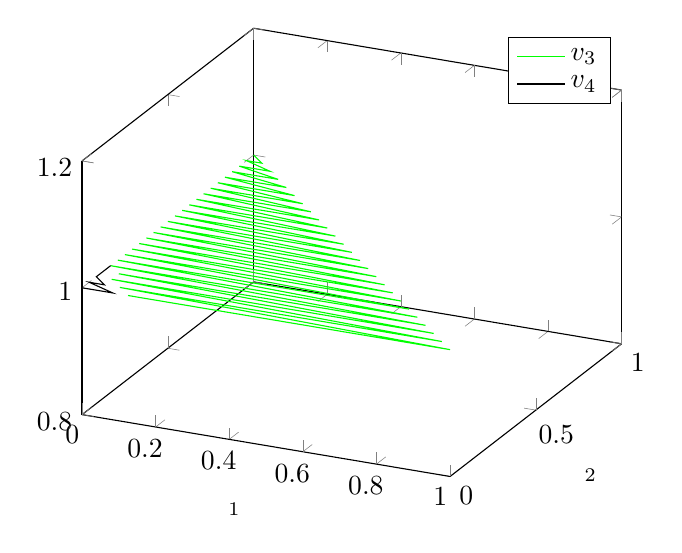
\begin{tikzpicture}
    \begin{axis}[
        xlabel=$\w_1$,
        ylabel=$\w_2$,
        domain=0:1,
        y domain=0:1
      ]

      % \addplot3[mark=none,color=pink]{-6*y + 3\geq=max(-6*y + 3,-x-4*y + 4,-5*x*-8*y + 10,-9*x-6*y + 11,-11*x-2*y + 9,-9*x+ 6)-0.1?1:NaN};
      % \addplot3[mark=none,color=blue]{-x-4*y + 4>=max(-6*y + 3,-x-4*y + 4,-5*x*-8*y + 10,-9*x-6*y + 11,-11*x-2*y + 9,-9*x+ 6)-0.1?1:NaN};
      \addplot3[mark=none,color=green]{x+y<=1 && -5*x*-8*y + 10>=max(-6*y + 3,-x-4*y + 4,-5*x*-8*y + 10,-9*x-6*y + 11,-11*x-2*y + 9,-9*x+ 6)?1:NaN};
      \addplot3[mark=none,color=black]{x+y<=1 && -9*x-6*y + 11>=max(-6*y + 3,-x-4*y + 4,-5*x*-8*y + 10,-9*x-6*y + 11,-11*x-2*y + 9,-9*x+ 6)?1:NaN};
      \addplot3[mark=none,color=red]{x+y<=1 && -11*x-2*y + 9>=max(-6*y + 3,-x-4*y + 4,-5*x*-8*y + 10,-9*x-6*y + 11,-11*x-2*y + 9,-9*x+ 6)?1:NaN};
      \addplot3[mark=none,color=blue]{x+y<=1 && -9*x+ 6>=max(-6*y + 3,-x-4*y + 4,-5*x*-8*y + 10,-9*x-6*y + 11,-11*x-2*y + 9,-9*x+ 6)?1:NaN};

      % \legend{$v_1$,$v_2$,$v_3$,$v_4$,$v_5$,$v_6$}
      \legend{$v_3$,$v_4$,$v_5$,$v_6$}
    \end{axis}
  \end{tikzpicture}

\end{figure}
\end{document}